\documentclass[11pt]{article}

\usepackage[a4paper,margin=2.45cm]{geometry}
\usepackage[T1]{fontenc}
\usepackage[utf8]{inputenc}
\usepackage{lmodern}
\usepackage{amsmath,amssymb}
\usepackage{booktabs,threeparttable,longtable,array,tabularx}
\usepackage{graphicx,float}
\usepackage{caption}
\usepackage{setspace}
\usepackage{enumitem}
\usepackage{microtype}
\usepackage[colorlinks=true,linkcolor=black,citecolor=black,urlcolor=blue]{hyperref}
\usepackage[backend=biber,style=authoryear-comp,maxcitenames=2,maxbibnames=99,uniquelist=false]{biblatex}
\addbibresource{../green_credit_transition_refs.bib}
\addbibresource{local_refs.bib}
\renewcommand*{\bibfont}{\small}

\captionsetup{font=small,labelsep=quad}
\setlength{\tabcolsep}{4pt}
\renewcommand{\arraystretch}{1.13}
\onehalfspacing
\setlist{nosep,leftmargin=2em}
\setlength{\emergencystretch}{2em}
\newcommand{\note}[1]{\begin{minipage}{0.96\textwidth}\footnotesize\textit{Notes:} #1\end{minipage}}

\title{Designed for Adjustment:\\
Coal-Power Lock-in and the Missing Exit Pathway in China, 2000--2023}
\author{Anonymous manuscript for review}
\date{}

\begin{document}
\maketitle

\begin{abstract}
Coal transition is often inferred from changes in energy intensity, emissions, or the coal share of energy use. Those measures do not show whether coal-power assets have retired. This study uses a 31-province panel for 2000--2023, reconstructed coal, wind, and solar project histories from Global Energy Monitor trackers, and coal-unit retirement records to examine China's transition architecture. It distinguishes operating, compositional, and asset-exit margins. More coal-exposed provinces recorded post-2012 declines in coal-use intensity and in coal's share of five-energy final use. The intensity estimates are sensitive to pre-trends and province-specific trends, so they are not interpreted as the causal effect of a single policy. The survival specifications show no statistically detectable acceleration of coal-unit retirement in high-coal-exposure provinces. Reconstructed national coal-power operating capacity rose from about 686~GW in 2011 to 1,143~GW in 2023, even as wind and solar capacity expanded. The national composition also changed: coal's share of the five-energy final-use basket fell from 68.2\% in 2006 to 58.8\% in 2022, while thermal capacity and generation shares declined. Operating and compositional transition therefore coexisted with continued asset accumulation. Direct coal-unit lifecycle evidence reveals an adjustment--exit gap: progress in coal use and energy-system composition does not by itself show a transition in the installed coal-asset stock. The findings do not identify one causal mechanism for this configuration. They indicate that a credible long-run transition architecture must connect adjustment with replacement, retirement, grid integration, and local fiscal and labour adjustment.
\end{abstract}

\noindent\textbf{Keywords:} coal-power retirement; carbon lock-in; policy design; energy transition; transition finance; China; just transition

\section{Introduction}

Energy transition is often assessed through carbon intensity, fuel shares, renewable investment, or pollutant emissions. These measures matter, but they leave a separate question unanswered: have incumbent fossil assets exited? Research on carbon lock-in and socio-technical transitions shows why decarbonization rarely amounts to simple replacement. Durable technologies, institutions, and policy feedback can preserve an incumbent system even as its operation changes \parencite{unruh2000,geelsschot2007,markardetal2012}. The coal-phaseout literature provides the starting point for this paper. Paris-consistent pathways limit the remaining operating lives of coal units, and plant-level studies set out possible retirement sequences for China \parencite{cui2019,cui2021}. Recent China-specific system modelling also shows that, under a binding carbon constraint, coal power can move from high-utilisation baseload generation to a flexibility role while retirement and carbon-capture decisions are jointly optimised \parencite{an2025}. This paper asks a different question: whether observed transition has reached the asset-exit margin. A coal generator may use less coal per unit of output, run fewer hours, install pollution-control equipment, or be supplemented by renewable generation and still remain in service. For long-lived plants, changing operation and retiring assets are different policy tasks \parencite{kefford2018}.

Operating adjustment, compositional change, and asset exit require different decisions and different evidence. Environmental regulation and transition finance can redirect innovation, lending, and operating practice \parencite{acemogluetal2012,campiglio2016}. Lower energy intensity may reflect technical improvement, changes in output composition, denominator growth, or the relocation of energy-intensive activity. A lower coal share may follow the expansion of electricity, gas, or renewables while coal generators remain in place. These indicators observe flows, rates, or system composition; they do not directly observe the lifecycle of the installed coal fleet. Exit, by contrast, requires retirement, cancellation, mothballing, or durable repurposing, together with decisions about closure, remediation, debt, replacement, and local-adjustment costs. Scenario studies of Chinese coal phaseout compare prioritised retirement with transition arrangements that retain part of the fleet as reserve or flexibility capacity during renewable expansion \parencite{cui2021,zhang2022phaseout,yin2021,an2025}. The empirical question here is narrower: whether observed operating and compositional adjustment has been accompanied by exit from the installed fleet.

China provides a useful case because renewable expansion has proceeded alongside continuing adequacy and integration requirements. Lower-carbon replacement depends on storage, transmission, hydro flexibility, dispatch reform, and renewable absorption, not only on additional wind and solar capacity \parencite{he2016,he2020,liu2019,davidson2016}. A lower thermal-generation share therefore does not settle the fate of a coal unit that may still provide capacity, flexibility, or reliability services \parencite{yin2021,an2025}. Exit costs are also geographically concentrated. Coal reliance varies across provinces in employment, fiscal, industrial, and power-system terms, so retirement is a regional-governance problem as well as a plant-level decision \parencite{jiang2023,greengambhir2020,hansencoenen2015}.

The Chinese green-credit framework forms part of this institutional context; it is not a stand-alone retirement programme. The 2012 Green Credit Guidelines placed environmental and social risk within bank lending practice \parencite{cbrc2012}, while research on the policy documents its environmental-finance rationale and uneven implementation \parencite{aizawayang2010,zhangyangbi2011}. The broader 2012--2023 policy mix included instruments for efficiency improvement, cleaner utilization, renewable deployment, and reliability. On their own, such instruments do not allocate the costs of retiring viable but carbon-intensive units, secure replacement services, or arrange fiscal and labour adjustment. This describes the tasks the instruments can coordinate. It does not attribute intent or a causal effect to any single policy or policymaker.

The post-2012 period provides a window for asking whether operating-margin transition was accompanied by asset exit. The Green Credit Guidelines and later national policies are not treated as province-level interventions with clean untreated comparisons. The provincial credit measure does not observe lending to coal assets, the bank-network instrument is weak, and a national policy date cannot separate finance from concurrent energy, industrial, and environmental policies. The absence of an automatic spillover does not show that any policy failed. It shows that improvements in operating and compositional measures cannot be assumed to establish fleet-wide retirement.

The analysis combines three forms of evidence. A balanced 31-province panel for 2000--2023 separates operating outcomes, coal-use composition, and thermal-power structure. Annual additions, retirements, and operating stocks of coal, wind, and solar are reconstructed from the Global Energy Monitor (GEM) trackers, along with retirement histories for 4,323 coal units. The GEM records directly observe the stock and lifecycle margin that intensity and share measures leave unresolved. They test whether changes in flows and shares have been accompanied by change in the installed coal fleet. We also map transition constraints using resource-linked employment, fiscal and industrial-asset exposure, coal-unit operating and standby requirements, renewable consumption, utilization, and project pipelines. Shanxi and Inner Mongolia are structured comparison cases rather than a causal two-province experiment.

The three margins moved at different speeds. In baseline specifications, more coal-exposed provinces had larger post-2012 declines in coal-use intensity and the coal share of final energy. Coal-share dynamics are comparatively clean, whereas intensity and selected pollutant results are sensitive to pre-trends or province-specific trends. Nationally, coal's share of the observed five-energy final-use basket fell from 68.2\% in 2006 to 58.8\% in 2022, while thermal capacity and generation shares also declined. Reconstructed coal-power operating capacity rose from 686~GW in 2011 to 1,143~GW in 2023, and the unit-level survival models do not detect faster retirement in high-coal-exposure provinces after 2012. This is adjustment--exit decoupling: operating and compositional indicators improved while coal assets continued to accumulate and retirement did not accelerate differentially. Renewable expansion did not automatically displace the coal fleet.

The paper calls this observable configuration \textit{lock-in through adjustment}. The concept separates \textit{greening the stock} from \textit{exiting the stock}: incumbent assets are cleaned, optimized, or functionally repositioned while no corresponding asset-exit pathway becomes visible in the evidence. It is an account of coexisting margins, not a claim that adjustment caused lock-in or that one policy instrument or provincial constraint caused the observed outcome.

The contribution is diagnostic rather than causal. The paper identifies where change occurs, at the operating, compositional, or asset margin, and asks whether the observed policy architecture connects those margins. This approach fits a setting where interventions overlap and the data describe regional systems more clearly than lender--borrower transactions. Measures that clean and optimize existing assets may meet their immediate purpose. A long-run transition architecture must also make retirement, replacement, grid integration, and local adjustment jointly feasible.

\section{Transition margins, path dependence, and coal-power exit}

The analysis distinguishes three margins of change. \textit{Operating adjustment} concerns changes within an incumbent system: fuel input per unit of output, utilization, pollutant emissions, and efficiency. \textit{Compositional adjustment} concerns the relative role of coal in final energy use or generation. \textit{Asset exit} concerns the retirement, cancellation, mothballing, or permanent repurposing of coal units. Operating and compositional indicators generally observe flows, rates, or shares; asset exit concerns the stock and lifecycle of incumbent infrastructure. The margins may move together, but they impose different coordination problems and are addressed by different instruments.

The distinction follows from policy-design and path-dependence theory. Policy mixes embody choices about objectives, instruments, and the distribution of adjustment costs \parencite{howlett2010}. Increasing returns can make an initially practical institutional arrangement self-reinforcing as infrastructure, capabilities, expectations, and compensation claims accumulate \parencite{arthur1989,pierson2000,mahoney2000}. Carbon lock-in similarly resides in the co-evolution of durable technical systems, institutions, and political-economic interests \parencite{unruh2000}. In this setting, environmental regulation and transition finance can affect operation without resolving retirement. Firms can improve technology, inputs, and abatement practices when environmental costs are internalized \parencite{portervanderlinde1995,popp2002,acemogluetal2012}; lenders can incorporate environmental risk into screening, pricing, covenants, and monitoring \parencite{stiglitzweiss1981,campiglio2016,dikauvolz2021}. Many of these responses are feasible within the life of an existing asset. They do not require the coordinated closure agreement that asset exit does.

This can produce a particular form of transition path dependence. Cleaner operation can reduce pollution and fuel use, and renewable additions can lower coal's share, while the retained fleet remains embedded in reliability arrangements, local tax bases, state-owned balance sheets, and employment systems. Transition may then proceed through regime-level optimization without dismantling or replacing the incumbent regime \parencite{geels2002,geelsschot2007,markardetal2012}. We call this observable configuration \textit{lock-in through adjustment}: the installed fleet becomes cleaner or less intensively used while the institutional conditions for exit remain unobserved. The term does not imply that adjustment is harmful or that it caused persistence. It describes why adjustment and exit may be decoupled rather than sequential.

Asset exit is more demanding. Coal generators are durable and capital-intensive. Their continued operation may support system adequacy, local employment, tax bases, and state-owned enterprise balance sheets. Their retirement can require replacement capacity, flexible generation or storage, transmission and dispatch arrangements, debt restructuring, land remediation, worker support, and fiscal adjustment. These complementarities make the relevant unit of transition larger than an individual lending decision. They also explain why the security-of-supply and build-before-breaking logic is reasonable in the short run, while still leaving a long-run design question: who provides the replacement service, bears the financial loss, and supports affected localities?

The distinction is institutional as well as technical. An adjustment-focused policy mix can succeed on its own terms when it improves operation, reduces local pollution, deploys renewables, and preserves adequate service. It does not establish an asset-exit pathway when retirement dates, retirement finance, replacement capacity, grid integration, and regional adjustment remain outside the policy package. These conditions need to be connected explicitly because exit redistributes costs across asset owners, workers, local governments, and electricity consumers \parencite{newellmulvaney2013}.

Regional conditions determine how acute these constraints are. Resource-linked employment, mining assets, taxes, and state industrial assets can raise the local cost of a rapid coal transition. At the same time, renewable resources and project development do not guarantee that renewable output can replace local coal generation. Grid access, consumption obligations, curtailment, storage, and interprovincial trade matter. The literature on regional capabilities similarly cautions that resource opportunities become new development paths only when they can be connected to knowledge, infrastructure, firms, and institutions \parencite{cohenlevinthal1990,hansencoenen2015,boschma2017}.

This perspective avoids treating provinces as simply brown or green. A province may be coal-dependent and possess excellent wind or solar resources. It may still retain coal assets if its development model depends on electricity exports, renewable output is curtailed or dispatched at low value, or coal generators retain a reliability role. A province with fewer local renewable resources may instead reduce coal capacity through trade and transmission. The empirical question is whether the observed asset trajectory is compatible with operating indicators and, where it is not, which constraints surround the divergence.

Operating and compositional adjustment can precede asset exit or occur without it. A gap between these margins does not show which constraint caused it. It does show that operating and compositional progress alone does not establish the exit margin. The analysis asks whether the margins moved together in China and describes the constraints around the observed divergence.

\section{Data and empirical approach}

\subsection{Provincial operating and constraint data}

The provincial panel contains 31 mainland provincial units for 2000--2023, or 744 province-year observations. It combines energy balances, generation and capacity data, emissions, macroeconomic indicators, resource-linked employment and fiscal measures, renewable-consumption indicators, monthly generation data, and provincial government-work-report text. The five-energy final-use measures cover coal, petroleum products, liquefied petroleum gas, natural gas, and electricity. They are useful for a consistent long panel but should not be described as total primary energy. The final-energy series ends in 2022; several power-system and renewable-consumption measures begin later. All tables report outcome-specific coverage.

The mixed coverage shapes what each source can do. Long historical series describe operating and compositional margins; the richest measures of reliability, renewable consumption, and utilization begin later. We do not backfill these later observations or treat them as pre-policy conditions. Instead, they describe the contemporary transition environment. The evidence is therefore layered: a long-run panel describes the operating pattern, project histories trace the asset trajectory, and later administrative measures describe conditions relevant to future exit.

The operating outcomes are final-energy intensity, final-coal intensity, the coal share of five-energy final use, selected industrial emissions, and thermal capacity and generation shares. Green total factor productivity and global Malmquist--Luenberger indices are not headline evidence because their production-function inputs cannot be fully reconstructed from the available source files. Resource-dependence measures use pre-policy mining employment, coal-mining assets, resource-tax revenue, and, in one extension, raw-coal output. Renewable-consumption reports cover all provinces from 2015, while coal-unit reliability indicators cover the 30 coal-unit provinces from 2018. Grid utilization and curtailment measures start later and have incomplete coverage. These measures describe constraints; they do not identify a pre-policy moderator.

\subsection{Direct asset evidence}

The asset data are reconstructed from the January 2026 Global Coal Plant Tracker, February 2026 Global Wind Power Tracker, and February 2026 Global Solar Power Tracker \parencite{gem2026}. For each Chinese project or unit with a recorded start and, where applicable, retirement year, annual provincial additions, retirements, and operating stocks are calculated. Coal coverage includes units of at least 30~MW; Tibet is absent from the source and is coded zero in the provincial panel. The current release identifies 4,323 coal units entering the retirement analysis and 952 retirements. The project histories are retrospective records from a 2026 snapshot rather than historical tracker vintages. Missing early start years imply that reconstructed early stocks should be interpreted as a lower bound.

The asset analysis has two parts. Descriptive trajectories show national and provincial additions, retirements, and reconstructed operating stock. A left-truncated Cox model then divides each coal unit's observed risk time into four calendar periods: 2000--2011, 2012--2015, 2016--2020, and 2021--2025. The specification controls for unit capacity and vintage, clusters uncertainty by province, and interacts period with pre-policy provincial coal exposure. It asks whether retirement hazards differed across coal-exposure areas over time. It is not a quasi-experiment for the Green Credit Guidelines.

Compared with a province-year retirement share, the survival design preserves the timing of retirement events and avoids treating a province with one very large closure as equivalent to one with many small unit retirements. It also conditions the comparison on plant capacity and vintage, both mechanically related to retirement risk. The design has important limits. Exposure is measured at the province rather than owner or plant level, policy periods are not random, and province-clustered uncertainty remains demanding with 30 coal-unit provinces. We therefore report the estimates as evidence on the location and timing of retirement, not as a test of a policy shock.

\subsection{Supporting provincial pattern}

For comparability with the prior analysis, we also estimate province and year fixed-effect models that interact a post-2012 indicator with the 2008--2011 provincial coal share in five-energy final use. Controls include log GDP, population, the secondary-industry share, urbanization, the environmental-expenditure share, and the marketization index. The coefficient describes a differential post-2012 association. Continuous-exposure event studies, province-specific trends, and alternative exposure measures serve as diagnostics. This remains supporting analysis because a national policy was implemented without an untreated province and several contemporaneous policies may have changed coal-intensive regions differently.

\begin{table}[H]
\centering
\small
\caption{Evidence architecture and inference boundary}
\label{tab:architecture}
\begin{tabularx}{\textwidth}{p{3.5cm}p{3.5cm}X}
\toprule
Evidence layer & Main measures & Permitted inference \\
\midrule
Asset exit & GEM additions, retirements, stocks; unit retirement histories & Direct evidence on whether coal assets exited. Retrospective source and observational comparison. \\
Operating adjustment & Energy and coal intensity, coal share, selected emissions & Differential provincial patterns, with explicit trend and construction limitations. \\
Transition constraints & Resource-linked employment, tax and assets; reliability; renewable consumption and utilization; project pipeline & Descriptive characterization of conditions associated with a difficult transition, not identified mechanisms. \\
Finance diagnostics & Provincial proxy and bank-network trial instrument & Explanation of why this paper does not make a local green-credit transmission claim. \\
\bottomrule
\end{tabularx}
\note{The unit of inference differs across rows. The study treats convergence across the evidence layers as a policy diagnosis, not as a single causal estimator.}
\end{table}

\section{Results}

\subsection{Coal capacity continued to grow while renewable capacity expanded}

The direct asset series describes the basic empirical setting. National reconstructed coal operating capacity rose from 686.3~GW in 2011 to 1,142.9~GW in 2023. Wind and solar operating capacity also rose from 43.6~GW to 722.6~GW over the same period. That expansion does not show that coal assets exited. Coal additions remained positive in every sample year. Retirements included several large closure waves, but they did not reduce the national operating stock.

Figure~\ref{fig:asset_lifecycle} shows the distinction directly. Annual coal retirements remained below annual commissioning in every year of the reconstructed 2000--2023 series. Net coal additions were therefore positive, including during rapid wind and solar expansion. The lower panel separates flows from stocks: wind and solar operating capacity rose rapidly, and the coal operating stock also increased. Renewable deployment was additive at the national level; it had not yet produced coal-asset exit.

\begin{figure}[H]
\centering
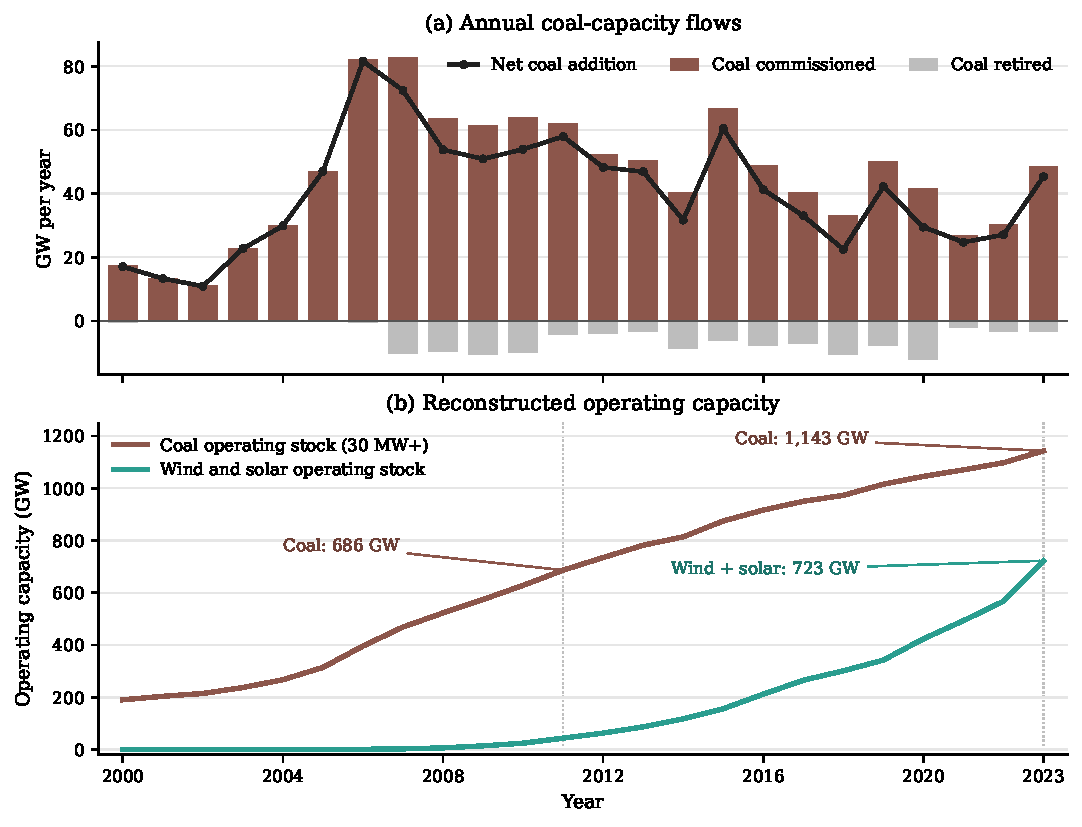
\includegraphics[width=\textwidth]{../../result/figures/energy_policy_lockin_0820/Figure_1_asset_lifecycle.pdf}
\caption{Coal additions, retirements, and operating stock alongside wind and solar expansion in China, 2000--2023}
\label{fig:asset_lifecycle}
\note{National sums are reconstructed from the January--February 2026 Global Energy Monitor tracker snapshots. Panel (a) reports annual coal capacity commissioned, retired, and net added. Panel (b) reports reconstructed operating capacity. Coal includes units of at least 30~MW. The histories are retrospective records based on reported start and retirement years; missing early start years imply that reconstructed early stocks are lower bounds.}
\end{figure}

This pattern changes how conventional structural indicators should be read. A stable or declining thermal-generation share can result from faster growth of total generation or renewables, changes in utilization, or new nonthermal capacity. None of these outcomes reveals whether coal units retired. The GEM histories show a system that accumulated renewable assets while retaining and expanding a large coal fleet.

\begin{table}[H]
\centering
\caption{Direct asset evidence on China's power transition}
\label{tab:assetfacts}
\begin{tabular}{lrr}
\toprule
Indicator & 2011 & 2023 \\
\midrule
Coal operating stock (GW) & 686.3 & 1,142.9 \\
Wind and solar operating stock (GW) & 43.6 & 722.6 \\
Coal capacity commissioned during year (GW) & 62.1 & 48.6 \\
Coal capacity retired during year (GW) & 4.2 & 3.3 \\
\bottomrule
\end{tabular}
\note{Stocks, additions, and retirements are reconstructed from GEM's 2026 tracker snapshot. Coal capacity is based on units of at least 30~MW. Values are national sums of province-year data and are rounded to one decimal place.}
\end{table}

The provincial distribution matters because coal capacity is concentrated in provinces with different resource dependence, grid roles, and renewable deployment. Some combine large coal fleets with large renewable portfolios; others retain coal capacity without comparable renewable absorption. The relevant question is whether particular regional systems have the conditions for replacement and retirement.

\subsection{High coal exposure did not show a detectable post-2012 retirement acceleration}

The retirement analysis does not show faster exit in coal-intensive provinces after 2012. Before 2012, one standard-deviation higher provincial coal exposure was associated with a hazard ratio of 1.26 for retirement ($p=0.063$). The estimated hazard ratio is 1.01 in 2012--2015 ($p=0.955$), 1.08 in 2016--2020 ($p=0.713$), and 1.12 in 2021--2025 ($p=0.613$). The estimates are imprecise. In the post-2012 policy window, the data do not detect a faster retirement hazard in more coal-exposed provinces. Hazard ratios near one, with confidence intervals spanning one, fit an observed adjustment--exit gap rather than a detectable differential movement into asset exit. They are not evidence that a policy intended to retire the fleet was ineffective.

Figure~\ref{fig:retirement_evidence} presents the result in two forms. The left panel tracks unadjusted cumulative retirement for units operating at the start of 2012, split at the median province-level coal exposure; the curves remain close through 2025. The right panel reports the corresponding calendar-period associations from the left-truncated Cox model after adjustment for capacity and vintage. The confidence intervals are wide, and each post-2012 interval includes a hazard ratio of one. The data do not show a detectable retirement acceleration in coal-exposed provinces and do not identify the cause of the observed pattern.

\begin{figure}[H]
\centering
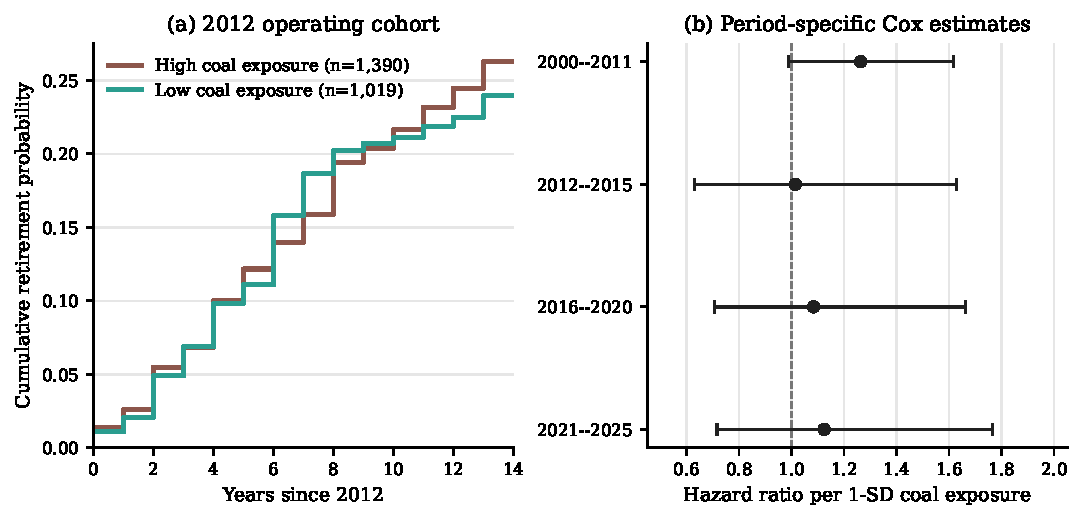
\includegraphics[width=\textwidth]{../../result/figures/energy_policy_lockin_0820/Figure_2_retirement_evidence.pdf}
\caption{Coal-unit retirement evidence by provincial coal exposure}
\label{fig:retirement_evidence}
\note{Panel (a) is an unadjusted Kaplan--Meier display for the 2,409 coal units operating at the start of 2012. High and low coal exposure are defined using the province-level median of pre-policy coal exposure. Panel (b) reports hazard ratios per one provincial standard deviation of pre-policy coal exposure from left-truncated Cox models with capacity and vintage controls; horizontal bars are 95\% confidence intervals using province-clustered robust standard errors. The displays are observational and do not identify a policy effect.}
\end{figure}

The province-year lifecycle regressions point in the same direction. Post-2012 coal exposure is not significantly associated with coal additions, coal retirements, net coal additions, or the reconstructed coal stock share. The absence of a detected differential does not prove that policy had no effect. It does show that a paper based only on energy intensity or coal shares would overstate structural change. Direct asset measures are needed to evaluate the exit margin.

\begin{table}[H]
\centering
\caption{Coal-unit retirement hazard by calendar period and pre-policy coal exposure}
\label{tab:cox}
\resizebox{\textwidth}{!}{%
\begin{tabular}{lrrrr}
\toprule
Period & Hazard ratio & Clustered SE of log hazard & $p$ value & Retirement events \\
\midrule
2000--2011 & 1.263 & 0.126 & 0.063 & 443 \\
2012--2015 & 1.014 & 0.241 & 0.955 & 135 \\
2016--2020 & 1.084 & 0.219 & 0.713 & 253 \\
2021--2025 & 1.124 & 0.230 & 0.613 & 121 \\
\bottomrule
\end{tabular}
}
\note{Left-truncated Cox model with 12,344 unit-period observations, capacity and vintage controls, and province-clustered standard errors. Coal exposure is standardized at the provincial level. Calendar-period contrasts are diagnostic and should not be read as causal policy tests.}
\end{table}

\subsection{Operating adjustment is visible, but it does not identify a single policy channel}

The supporting provincial panel provides the other half of the puzzle. In the baseline fixed-effect specifications, higher pre-policy coal exposure is associated with larger post-2012 reductions in five-energy final intensity ($-0.289$, $p=0.021$), final-coal intensity ($-0.426$, $p<0.001$), and the five-energy coal share ($-0.250$, $p=0.003$). The coal-share event study has no evidence of differential pre-trends ($p=0.840$). By contrast, the intensity event studies have joint pre-trend $p$ values of 0.052 and 0.041, and both estimates become statistically indistinguishable from zero once province-specific linear trends are added.

These diagnostics need a bounded interpretation. The data show operating and compositional adjustment in more coal-exposed provinces. They do not isolate the Green Credit Guidelines or show that declining emissions resulted from treatment investment rather than output, fuel, relocation, or other regulations. A lower coal share also does not establish coal-asset retirement. The operating results are diagnostic: they document change at operating and compositional margins without showing that those changes produced asset exit.

\begin{table}[H]
\centering
\caption{Supporting provincial evidence: operating and compositional adjustment}
\label{tab:operating}
\resizebox{\textwidth}{!}{%
\begin{tabular}{lrrrr}
\toprule
Outcome & Baseline coefficient & $p$ value & Pre-trend $p$ value & Province-trend coefficient \\
\midrule
Five-energy final intensity & -0.289 & 0.021 & 0.052 & -0.123 \\
Final-coal intensity & -0.426 & <0.001 & 0.041 & -0.057 \\
Five-energy coal share & -0.250 & 0.003 & 0.840 & 0.090 \\
Industrial SO$_2$ & -72.589 & 0.001 & 0.053 & 28.616 \\
\bottomrule
\end{tabular}
}
\note{Province and year fixed effects, province-clustered standard errors, 2007--2022 or 2007--2023 depending on outcome availability. Baseline coefficients are for Post-2012 $\times$ pre-policy coal exposure. The table is a diagnostic summary, not a causal policy-effect table.}
\end{table}

\subsection{Transition constraints are visible in the provincial setting}

The asset and operating evidence motivate an examination of the conditions around exit. Resource-linked fiscal and employment measures identify provinces where coal is embedded in local economic systems. Coal-unit reliability reports add an operational consideration: even when coal's annual share falls, operating and standby requirements can preserve units as capacity resources. Renewable-consumption and utilization measures add the demand-side constraint. New wind and solar capacity matters for transition only when generation can be absorbed, transmitted, stored, or used to replace thermal output rather than supplementing it.

Their coverage limits causal claims, but they remain useful for policy diagnosis. Renewable consumption is available for all provinces from 2015 through 2023. Coal-unit reliability measures cover 2018--2023. Wind and solar utilization measures mainly cover 2018--2023, and project-pipeline data are a 2026 status snapshot. These data cannot establish whether pre-policy grid conditions caused a later retirement decision. They show that coal exit depends on fiscal, labour, reliability, and absorption issues that an operating-intensity regression does not capture.

Figure~\ref{fig:constraint_typology} plots this bundle without turning it into a mechanism test. Provinces are placed by reconstructed coal operating stock and renewable-consumption share, while colour records pre-policy resource dependence. Shanxi and Inner Mongolia fall in the high-coal-stock, below-median renewable-consumption quadrant, but their resource-dependence profiles differ. The figure is a descriptive policy typology. It identifies combinations of transition conditions that call for different policy packages; it does not estimate the effect of an individual condition on retirement.

\begin{figure}[H]
\centering
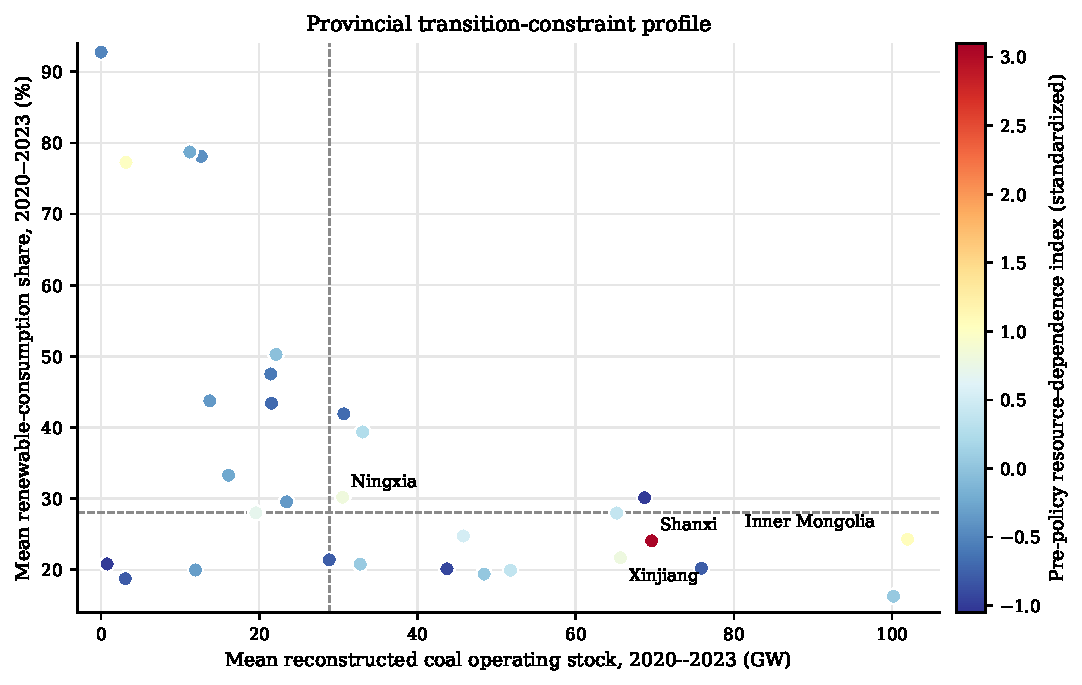
\includegraphics[width=\textwidth]{../../result/figures/energy_policy_lockin_0820/Figure_3_constraint_typology.pdf}
\caption{Descriptive provincial transition-constraint profile}
\label{fig:constraint_typology}
\note{Each point is a province. The horizontal axis is mean reconstructed coal operating stock and the vertical axis is mean renewable-consumption share, both over 2020--2023. Dashed lines mark the province medians. Colour denotes the standardized pre-policy resource-dependence index, constructed from mining employment, coal-mining assets, and resource-tax exposure where available. The figure is descriptive and should not be read as a causal classification or a retirement model.}
\end{figure}

Pipeline data caution against treating capacity shares as a complete measure of transition readiness. A large renewable pipeline may improve the feasibility of replacement, while an active coal construction or pre-construction pipeline can reproduce lock-in even as older units retire. Existing coal stock and prospective coal investment must be considered together. Likewise, a high renewable capacity share does not measure substitution when consumption and utilization remain constrained. These statements do not estimate the net effect of each variable.

Shanxi and Inner Mongolia illustrate two versions of an adjustment-first architecture. Figure~\ref{fig:case_lifecycles} shows that both accumulated wind and solar capacity while their coal operating stocks continued to grow. By 2023, reconstructed coal and wind-solar stocks were 74.3 and 42.8~GW in Shanxi, and 115.1 and 82.1~GW in Inner Mongolia. Shanxi combines a large coal stock with a strong coal-linked economic base. Inner Mongolia combines very large coal capacity with a larger wind and solar project system and an external-power orientation. Renewable endowment and resource dependence shape these configurations, but neither automatically supplies an exit pathway. The cases are not clean counterfactuals. Government-work-report text supports only a narrow contrast: after 2012, Inner Mongolia used more green-finance and clean-coal language than Shanxi, while differences in renewable-energy and pollution-control language are not statistically stable. The comparison describes different transition conditions; it does not prove a policy mechanism.

\begin{figure}[H]
\centering
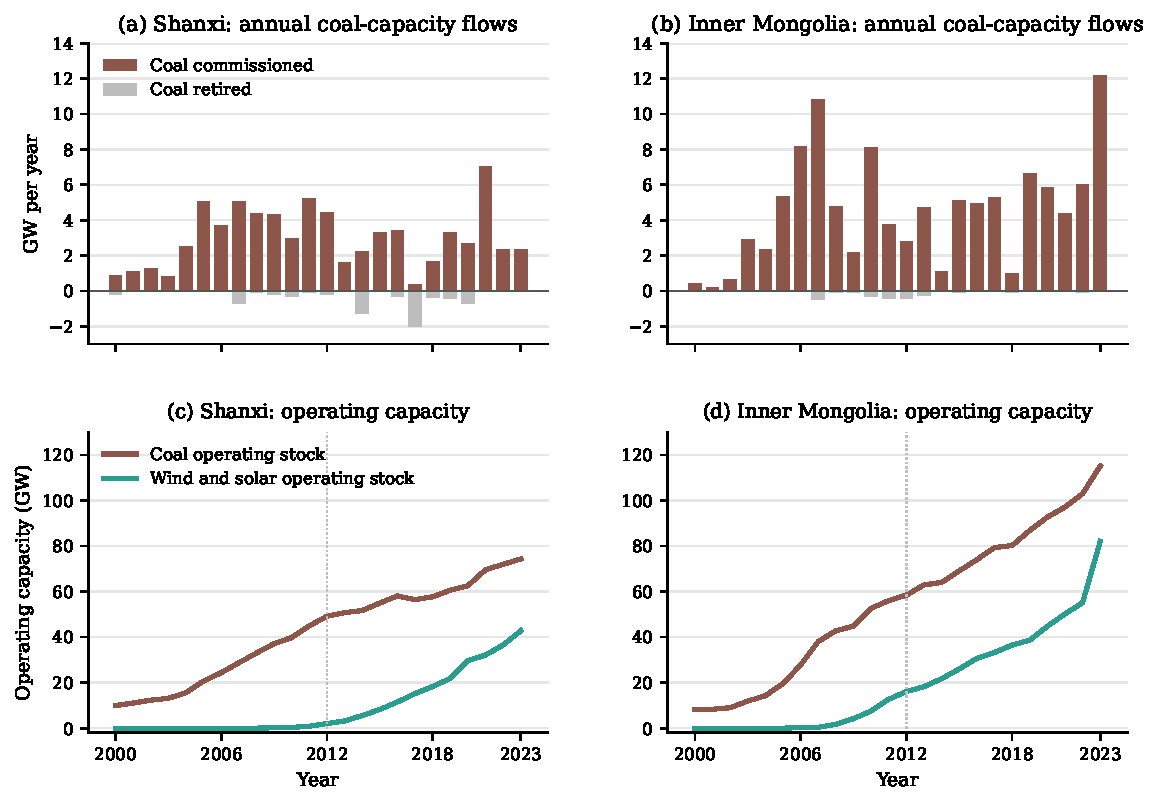
\includegraphics[width=\textwidth]{../../result/figures/energy_policy_lockin_0820/Figure_4_case_lifecycles.pdf}
\caption{Shanxi and Inner Mongolia: coal-capacity flows and operating stocks, 2000--2023}
\label{fig:case_lifecycles}
\note{Panels (a)--(b) report annual coal capacity commissioned and retired; panels (c)--(d) report reconstructed coal and wind-solar operating capacity. The vertical dotted line marks 2012. National tracker conventions apply: coal includes units of at least 30~MW, and historical stocks are reconstructed retrospectively from the 2026 GEM tracker snapshot. The case comparison is descriptive, not a causal two-province design.}
\end{figure}

Figure~\ref{fig:composition_shares} provides a national composition check with each denominator stated explicitly. In the observed five-energy final-use basket, coal's share declined from 68.2\% in 2006 to 58.8\% in 2022, while electricity and natural-gas shares increased. In the power system, thermal capacity fell from 77.6\% of installed capacity in 2006 to 47.6\% in 2023, and thermal generation fell from 80.9\% to 65.6\%. These changes are substantial, but non-thermal power is not synonymous with renewable power, and electricity in the final-use basket is not itself a clean-energy source. Shares also do not identify what happened to the pre-existing coal fleet. China experienced compositional transition alongside continued coal-asset accumulation.

\begin{figure}[H]
\centering
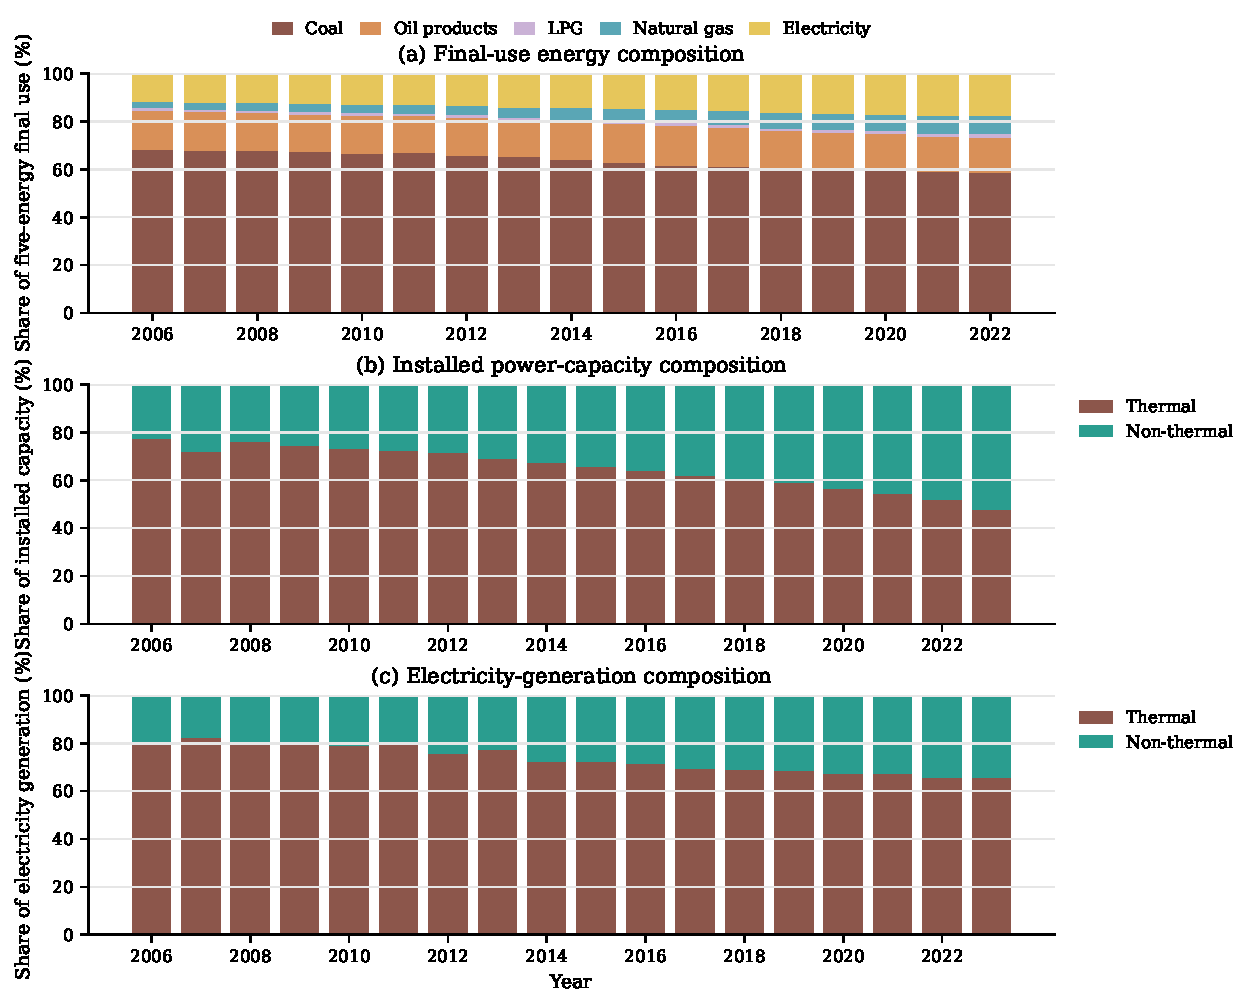
\includegraphics[width=\textwidth]{../../result/figures/energy_policy_lockin_0820/Figure_5_annual_composition_shares.pdf}
\caption{Annual energy and power-system composition, national provincial sums}
\label{fig:composition_shares}
\note{Panel (a) uses the five-energy final-use basket: coal, oil products, LPG, natural gas, and electricity. It is not a total-primary-energy measure, and electricity should not be interpreted as a clean-energy category. Panels (b) and (c) use total installed capacity and total generation, respectively; non-thermal includes all non-thermal sources, not only wind and solar. Values are annual sums across provinces before shares are computed. The panels describe composition and do not measure coal-unit retirement.}
\end{figure}

\subsection{Alternative interpretations and the scope of the evidence}

Coal capacity growth may reflect a security-of-supply response. This is plausible in a system facing demand growth, regional imbalance, and variable renewable output. The paper does not imply that every retained coal unit is irrational or should close immediately. It shows that a security rationale for retention has policy consequences that intensity measures do not reveal. If coal capacity is retained for reliability, an eventual exit pathway must specify the replacement service, its location, and the institution responsible for providing it.

The national stock trajectory might also be driven by a small number of provinces and say little about coal-intensive regions generally. The provincial survival analysis addresses this concern imperfectly but directly. It asks whether exposure to coal-intensive final energy use predicts a differential retirement pattern. The data do not reveal a post-2012 acceleration. The inference remains observational, but it connects the exit margin to the regional distribution of coal dependence in a way that a national capacity series cannot.

The operating pattern may be driven by policies unrelated to finance, including energy-conservation targets, coal-consumption controls, air-pollution action plans, industrial restructuring, or supply-side reform. This is a substantive limitation. These policies often acted on the same coal-intensive regions and may have shared implementation channels. The operating pattern is consistent with a period of tighter constraints on coal-intensive activity. It cannot be assigned to green credit or used to claim that finance alone explains the absence of asset exit.

Renewable additions can contribute to decarbonization even when they do not retire coal units immediately. The policy question is whether those additions form part of a pathway that eventually changes the coal fleet. Direct asset data make that question observable over time. They distinguish additive renewable deployment from deployment linked to a credible schedule of replacement and retirement.

\section{Discussion: connecting adjustment to exit}

The policy implication concerns sequencing, not a verdict of policy failure. Efficiency standards, environmental enforcement, cleaner utilization, renewable investment, and reliability measures can reduce coal use at the operating margin while maintaining adequate electricity service. The evidence is consistent with operating and compositional transition, even though it does not isolate the effect of one instrument. Deep decarbonization requires a disposition of unabated coal assets. The policy problem is that adjustment today has no automatic institutional connection to exit tomorrow.

The long-run problem is an adjustment--exit gap. Cleaner operation and renewable additions do not determine when an existing generator retires. When closure costs fall on asset owners, local governments, workers, and system operators, a system can improve its indicators while retaining assets whose eventual disposition remains unresolved. This does not show that adjustment-oriented policies failed. It identifies a policy-task boundary: instruments that govern the operation of incumbent assets do not by themselves govern their retirement. A credible long-run transition architecture must connect the operating margin to replacement and retirement.

An architecture that connects adjustment to exit has four linked elements. First, it requires credible retirement or repurposing pathways, including owner-level transition plans, debt resolution, compensation rules, and safeguards against refinancing new coal expansion. Retirement finance is not a generic green-finance product; it must be tied to verifiable closure, remediation, and replacement milestones. Second, it requires dependable replacement capacity. Demand response, storage, flexible low-carbon generation, transmission, and market arrangements must supply the energy, capacity, and flexibility services previously provided by coal. This is the operational content that makes a build-before-breaking principle credible rather than rhetorical.

Exit also requires local fiscal and labour adjustment. Resource-tax dependence, mining employment, and state-owned industrial assets make retirement a regional-development issue as well as a plant-level transaction. Policies that leave these costs wholly local may favour continued operation or new construction. Renewable investment must also be connected to grid absorption and dispatch. Capacity targets alone do not ensure that renewable generation displaces coal generation; consumption, transmission, storage, and dispatch rules determine whether new assets substitute for the incumbent stock. These elements are complementary. Moving one forward while ignoring the others can reproduce the adjustment--exit gap.

The observed configuration also suggests a dynamic risk that this study does not test. Conventional lock-in is inherited from past investment, infrastructure, employment, fiscal dependence, and reliability arrangements. Under some conditions, transition-oriented adjustment may renew rather than merely inherit these commitments. Retrofit investment, functional repositioning as flexibility or capacity resources, and new revenue or institutional arrangements may reduce the short-run cost of retaining a coal unit while extending its economic or system value. The same investments that make an incumbent asset easier to retain today may therefore make its eventual retirement harder to coordinate tomorrow. This is not a sunk-cost claim, and the present data do not observe unit-level retrofit dates, capital expenditure, debt, or post-retrofit retirement responses. It is a theoretical implication and a future empirical proposition concerning unrecovered capital, renewed asset value, and institutional complementarity \parencite{arthur1989,pierson2000,mahoney2000,unruh2000}.

The data allow only a limited green-credit interpretation. Finance remains relevant because lending conditions affect new coal construction, retrofit, renewable investment, and the viability of closure transactions. The study neither observes bank-to-plant lending nor identifies a sufficiently strong province-by-bank credit shock. It cannot show that green credit caused the observed operating changes or that green credit failed. Financial and environmental measures directed at coal use may advance operating and compositional adjustment, but they do not complete an asset transition on their own.

The analysis has several limitations. GEM's histories are reconstructed from a current tracker release and may understate early capacity where start dates are missing. The survival estimates are observational and contain a limited number of province clusters. Provincial operating measures do not resolve all difference-in-trends concerns, and some constraint data start well after the 2012 policy break. The study also cannot measure owner debt, plant profitability, local capacity-market arrangements, or worker outcomes directly. These are not minor omissions; they identify the next data requirements for causal work on coal exit.

Future causal research on financial transmission would require bank-by-province pre-policy lending weights, bank-specific changes in green and high-carbon lending, and owner or plant-level debt and retirement information. Research on grid constraints would require historically comparable provincial transmission, dispatch, and power-trade data. Until those data are assembled, the evidence can distinguish the observed transition problem from possible mechanisms but cannot identify one mechanism from a national policy date.

\section{Conclusion}

Operating and compositional indicators alone cannot assess China's transition. Reductions in coal-use intensity and coal's share of energy coexist with a growing coal-power operating stock and no detected acceleration of retirement in high-coal-exposure provinces. The distinction separates a transition in flows and shares from a transition in the lifecycle of installed assets.

The evidence does not attribute this pattern to green credit or another single national policy. It identifies an adjustment--exit boundary that becomes visible only when direct asset evidence is read alongside operating and composition data. The 2012--2023 policy mix included instruments relevant to operating adjustment, cleaner utilization, renewable expansion, and adequate supply. The lack of automatic asset exit does not show that these instruments failed at their immediate tasks. It shows that progress on those tasks cannot demonstrate that the installed coal fleet has entered an exit pathway.

Measures directed at coal use may succeed on their own terms, but they cannot complete a transition that requires asset exit. A credible long-run strategy must join adjustment, replacement, retirement, grid integration, and local fiscal and labour adjustment. China has begun to transition at the operating and compositional margins. Whether its institutions will connect that adjustment to an orderly exit pathway for the coal fleet remains unresolved.

\section*{Data availability}
The provincial panel, processing scripts, regression outputs, and derived project-lifecycle measures are available from the authors upon reasonable request, subject to the redistribution terms of the underlying Wind and Global Energy Monitor data. Public source records and variable-coverage files are documented in the replication materials. The Global Energy Monitor tracker data are cited in the reference list.

\section*{Declaration of competing interests}
The authors declare that they have no known competing financial interests or personal relationships that could have appeared to influence the work reported in this paper. \textit{This statement must be confirmed by all authors before submission.}

\section*{Funding}
This research did not receive any specific grant from funding agencies in the public, commercial, or not-for-profit sectors. \textit{Replace this sentence if any author received relevant funding.}

\section*{Declaration of generative AI and AI-assisted technologies in the manuscript preparation process}
During the preparation of this work, the authors used OpenAI Codex for manuscript organization and language drafting. After using this tool, the authors reviewed and edited the content as needed and take full responsibility for the content of the published article. \textit{All authors must verify that this statement accurately reflects their use before submission.}

\printbibliography

\end{document}
